
\section{Planung und Konzeption}
Um später die Spiellogik zu implementieren musste zunächst der grobe Spielablauf analysiert werden. Zum Spielablauf gehören: Das Spiel starten, pausieren, gewinnen, verlieren und das Spiel neu starten. Daraus ergibt sich der folgende Automat:\\
\begin{figure}[ht]
	\centering
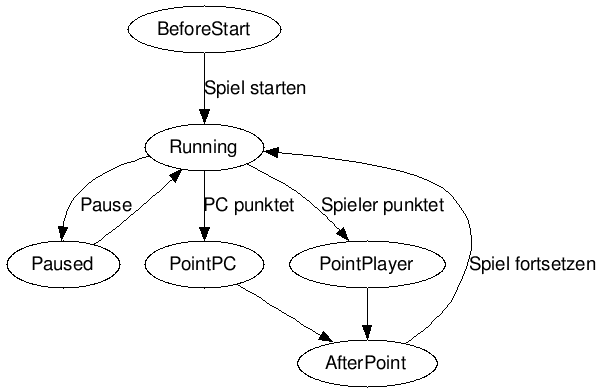
\includegraphics[width=0.33\textwidth]{fsm.png}
\caption{Spielzustands-Automat}
\end{figure}\\\\
Zur Umsetzung des Spiels müssen im wesentlichen Die vier Wände, der Ball und die Schläger gezeichnet werden. Des weiteren müssen das aktuelle Level (In Form von Schädeln) und die aktuelle Anzahl der Extra-Leben (als Herzen) angezeigt werden. Wird das Spiel gestartet, kann der Schläger mit der Maus gesteuert und der Ball mit Enter gestartet werden. Berührt der Ball einen Schläger muss je nach Geschwindigkeit des Schlägers die Flugbahn des Balls angepasst werden. Ebenfalls wird bei jeder Kollision ein zufälliger Sound abgespielt. \\
Verlässt der Ball das Spielfeld auf der Seite des Gegners, gewinnt der Spieler und der Schwierigkeitsgrad erhöht sich. Dies zeigt sich an einem schnelleren Ball und einem besser reagierenden Computergegner.\\
Verlässt der Ball das Spielfeld auf der Seite des Spielers, so wird ein Extra-Leben angezogen. Erreicht die Anzahl der Leben null, so gilt das Spiel als verloren und beginnt von vorne.\\\\
Die Umsetzung des Programms wurde grob in folgende Milestones geteilt:\\
\begin{itemize}
	\item Darstellung des Spielfeldes
	\item Bewegung der Schläger und einfache Flugbahn des Balls
	\item Umsetzung des HUDs
	\item Umsetzung der Bonusaufgaben
	\subitem Realistische Flugbahn des Balls
	\subitem Sounds und Musik
	\item Feinschliff
	\item Erstellung der Dokumentation
\end{itemize}
Da die ersten drei Punkte innerhalb 2 bis 3 Tagen bereits erledigt waren, wurden keine festen Daten zum erreichen der restlichen Milestones festgelegt. Da das Projekt über GIT organisiert wurde, konnte jederzeit ohne weitere Absprache am Projekt weitergearbeitet werden. Mindestens ein mal pro Woche wurde darüber Rücksprache gehalten, wie das weitere Vorgehen aussieht.